\documentclass[]{article}
\usepackage[a4paper,top=3cm,bottom=2.5cm,left=2.5cm,
            right=2cm,marginparwidth=1.75cm,
            headheight=5pt]{geometry}
\usepackage[T5]{fontenc}
\usepackage[utf8]{inputenc}
\usepackage[document]{}
\usepackage[vietnamese]{babel}
\usepackage[unicode]{hyperref}
\usepackage{amsmath}
\usepackage{setspace}
\usepackage{graphicx}
\usepackage{caption}
\usepackage{subcaption}
\usepackage{tcolorbox}
\usepackage{listings}
\usepackage{hyperref}
\usepackage{xcolor}
\usepackage{longtable}
\usepackage{titlesec}
\usepackage{floatrow}
\usepackage[nottoc]{tocbibind}
\usepackage{mdframed}
\usepackage{amsmath}
\usepackage{amssymb}
\usepackage{tgbonum}
\usepackage{type1cm}
\usepackage{indentfirst}
\usepackage{lettrine}
\usepackage{colortbl}
\usepackage{fancyhdr}
\usepackage{wrapfig}
\usepackage{lastpage}
\usepackage{url}
\addto\captionsenglish{
  \renewcommand{\contentsname}{MỤC LỤC}%
  \renewcommand{\listfigurename}{Danh sách ảnh}%
  \renewcommand{\listtablename}{Danh sách bảng}%
  \renewcommand{\figurename}{Hình}
  \renewcommand{\tablename}{Bảng}
}
\pagestyle{fancy}
\fancyhf{}
\rhead{Toán ứng dụng và thống kê}
\lhead{\color{cyan}Đồ án 3: Linear Regression}
\lfoot{Trang \thepage /\pageref{LastPage}}
\renewcommand{\footrulewidth}{0.4pt}
\setlength{\parindent}{1.5em}
\setlength{\parskip}{1cm}
\renewcommand{\baselinestretch}{1.5}
\newmdenv[linecolor=black,skipabove=\topsep,skipbelow=\topsep,
leftmargin=2.5cm,rightmargin=2.5cm,
innerleftmargin=5cm,innerrightmargin=5cm]{mybox}
\usepackage{multicol}
\usepackage{indentfirst}
\usepackage{color}
\usepackage{tikz}
\graphicspath{{Figures/}} 
\usepackage{lipsum}
\usetikzlibrary{calc}
\setlength{\columnseprule}{2pt}
\def\columnseprulecolor{\color{black}}
\def\maru#1{\textcircled{\scriptsize#1}}

\usepackage[backend=biber, style=numeric]{biblatex}
\addbibresource{refs.bib} % Tải tệp references.bib
\defbibheading{mybibintoc}{\section{Tài liệu tham khảo}}


\begin{document}

% Bìa trang
\begin{titlepage}
\begin{tikzpicture}[remember picture,overlay,inner sep=0,outer sep=0]
     \draw[blue!70!black,line width=4pt] ([xshift=-1.5cm,yshift=-2cm]current page.north east) coordinate (A)--([xshift=2cm,yshift=-2cm]current page.north west) coordinate(B)--([xshift=2cm,yshift=2cm]current page.south west) coordinate (C)--([xshift=-1.5cm,yshift=2cm]current page.south east) coordinate(D)--cycle;

     \draw ([yshift=0.5cm,xshift=-0.5cm]A)-- ([yshift=0.5cm,xshift=0.5cm]B)--
     ([yshift=-0.5cm,xshift=0.5cm]B) --([yshift=-0.5cm,xshift=-0.5cm]B)--([yshift=0.5cm,xshift=-0.5cm]C)--([yshift=0.5cm,xshift=0.5cm]C)--([yshift=-0.5cm,xshift=0.5cm]C)-- ([yshift=-0.5cm,xshift=-0.5cm]D)--([yshift=0.5cm,xshift=-0.5cm]D)--([yshift=0.5cm,xshift=0.5cm]D)--([yshift=-0.5cm,xshift=0.5cm]A)--([yshift=-0.5cm,xshift=-0.5cm]A)--([yshift=0.5cm,xshift=-0.5cm]A);


     \draw ([yshift=-0.3cm,xshift=0.3cm]A)-- ([yshift=-0.3cm,xshift=-0.3cm]B)--
     ([yshift=0.3cm,xshift=-0.3cm]B) --([yshift=0.3cm,xshift=0.3cm]B)--([yshift=-0.3cm,xshift=0.3cm]C)--([yshift=-0.3cm,xshift=-0.3cm]C)--([yshift=0.3cm,xshift=-0.3cm]C)-- ([yshift=0.3cm,xshift=0.3cm]D)--([yshift=-0.3cm,xshift=0.3cm]D)--([yshift=-0.3cm,xshift=-0.3cm]D)--([yshift=0.3cm,xshift=-0.3cm]A)--([yshift=0.3cm,xshift=0.3cm]A)--([yshift=-0.3cm,xshift=0.3cm]A);

   \end{tikzpicture}
\newcommand{\HRule}{\rule{\linewidth}{0.5mm}}
\center

\textsc{\Large TRƯỜNG ĐẠI HỌC KHOA HỌC TỰ NHIÊN}\\[0.5cm]
\textsc{\Large KHOA CÔNG NGHỆ THÔNG TIN}\\[1cm]

\includegraphics[width=0.3\textwidth]{logo/KHTN.jpg}\\[1cm]

\HRule \\[0.4cm]
{\huge \bfseries ĐỒ ÁN 3: LINEAR REGRESSION} \\[0.4cm]
{\large TOÁN ỨNG DỤNG VÀ THỐNG KÊ}\\[0.1cm]
\HRule \\[1.5cm]

\centerline{\Large{\textbf{Triệu Nhật Minh — 21127112 — 21CLC02}}}
\vspace{2.5cm}
\centerline{\large{\textit{Giảng viên hướng dẫn}}}
\vspace{0.25cm}
\centerline{\large{Vũ Quốc Hoàng}}
\centerline{\large{Lê Thanh Tùng}}
\centerline{\large{Nguyễn Văn Quang Huy}}
\centerline{\large{Phan Thị Phương Uyên}}

\vspace{2.5cm}
\centerline{\today}


\vfill % Wipe blank space of the page.
\end{titlepage}

% Mục lục tự động
\setlength{\parskip}{.7em}
\tableofcontents
\newpage

% Table of Figures & Tables
\setlength{\parskip}{.5em}
%\listoffigures
%\listoftables
\newpage

% Bắt đầu nội dung

\section{Thư viện sử dụng}
\subsection{pandas}
Thư viện cho phép thao tác với dữ liệu dạng bảng. pandas cung cấp các đối tượng DataFrame và Series, cho phép lưu trữ, truy xuất, lọc, nhóm, biến đổi và thống kê dữ liệu một cách hiệu quả và dễ dàng. Trong đồ án này, pandas được sử dụng để đọc dữ liệu từ file csv và lưu trữ dữ liệu dưới dạng DataFrame.

\subsection{numpy}
Thư viện cho phép thao tác với mảng nhiều chiều. Với bài toán data fitting sử dụng phương pháp bình phương tối thiểu (OLS Linear Regression), để giải nghiệm \textit{x} cho hệ phương trình được tính bằng công thức $\text{x} = (\text{A}^\text{T} \text{A})^{-1} \text{A}^\text{T} \text{b}$. Nhằm tối ưu thời gian tính toán, ta sử dụng hàm có sẵn từ thư viện này. Hầu hết các hàm có sẵn đã quen thuộc từ những đồ án trước, duy có hàm \textit{numpy.ravel} và \textit{numpy.triu} sẽ được giải thích rõ hơn ở phần liệt kê hàm.

\subsection{matplotlib}
Thư viện matplotlib (cụ thể là module pyplot) cho phép ta tạo ra các biểu đồ dạng 2D. matplotlib.pyplot cũng cho phép điều chỉnh các thuộc tính của đồ thị, như màu sắc, kích thước, chú thích và tiêu đề cho đồ thị. 

\subsection{seaborn}
Thư viện cho phép vẽ heatmap. Heatmap là một loại biểu đồ 2D biểu diễn giá trị của một ma trận bằng cách sử dụng các ô có màu sắc khác nhau. seaborn cung cấp các hàm để vẽ heatmap từ các đối tượng DataFrame hoặc numpy array, cũng như điều chỉnh các thuộc tính như bản đồ màu, khoảng giá trị, nhãn và tiêu đề. Heatmap là thành phần không thể thiếu để tìm hiểu mối quan hệ giữa các biến trong bộ dữ liệu và là tiền đề để thực hiện tìm mô hình cho yêu cầu 1d.

\subsection{sklearn}
Thư viện cho phép chia dữ liệu thành các fold để thực hiện cross-validation. Cross-validation là một kỹ thuật kiểm tra hiệu năng của mô hình học máy bằng cách sử dụng một phần của dữ liệu làm tập kiểm tra và phần còn lại làm tập huấn luyện. \textit{sklearn.model\_selection.KFold} cho phép chia dữ liệu thành k fold có kích thước bằng nhau và lặp qua từng fold để sử dụng làm tập kiểm tra hoặc tập huấn luyện.

\textit{sklearn.model\_selection.KFold} là một lớp trong thư viện scikit-learn, cung cấp các chỉ số để chia dữ liệu thành các tập huấn luyện và kiểm tra. Nó chia tập dữ liệu thành k fold liên tiếp. Mỗi fold được sử dụng một lần làm tập kiểm tra trong khi các fold còn lại được sử dụng làm tập huấn luyện.

Hàm tự cài đặt có thể thực hiện chức năng tương tự như KFold, nhưng có thể khác biệt về hiệu suất và tính năng. Việc sử dụng KFold từ scikit-learn có thể đảm bảo tính ổn định và độ tin cậy của kết quả, do nó được sử dụng rộng rãi trong cộng đồng khoa học dữ liệu, nhất là khi bộ dữ liệu được sử dụng trong đồ án khó có thể kiểm tra thủ công. Tuy nhiên, một hàm tự cài đặt có thể được tùy chỉnh để phù hợp với nhu cầu đặc biệt của người dùng, thậm chí có thể có hiệu suất tốt hơn so với KFold trong một số ít trường hợp.

\subsection{IPython}
Thư viện này không đóng góp vào việc giải quyết bài toán, nhưng vẫn được sử dụng vì khả năng hiển thị ngôn ngữ LaTeX để trình bày công thức hồi quy tuyến tính cho yêu cầu 1a do số lượng biến lớn. Module IPython.display.Latex cho phép chèn các biểu thức LaTeX vào Jupyter Notebook.

\section{Hàm sử dụng}
% Template
% \noindent
% \textbf{Input:} \\
% \textbf{Output:}
% \paragraph{Mô tả:}
\subsection{Hàm built-in từ thư viện}
% Pandas
\subsubsection{Hàm pandas.read\_csv}
\noindent
\textbf{Input:} Đường dẫn đến file csv. \\
\textbf{Output:} DataFrame chứa dữ liệu từ file csv.
\paragraph{Mô tả:}

Hàm \textit{pandas.read\_csv} \cite{pandasreadcsv} được sử dụng để đọc dữ liệu từ file csv và lưu trữ dữ liệu dưới dạng DataFrame. Hàm này có thể nhận thêm các tham số để tùy chỉnh cách đọc dữ liệu, nhưng trong đồ án này ta giữ nguyên các tham số khác xem như mặc định, chỉ tùy chỉnh đường dẫn đến file csv.

\subsubsection{Hàm pandas.drop}
\noindent
\textbf{Input:} Tên cột cần xóa. \\
\textbf{Output:} DataFrame sau khi đã xóa cột.

\paragraph{Mô tả:}
Trong yêu cầu 1d, để xây dựng mô hình chứa các đặc trưng chứa ít sự tương quan nhát (least correlation features), sau khi đã tìm được ma trận tương quan giữa các cột, ta sẽ xóa các cột có độ tương quan cao hơn 0.6. Mặc dù trong cộng đồng khoa học dữ liệu, các đặc trưng có độ tương quan cao hơn 0.95 mới được xem là có sự tương quan cao, nhưng trong đồ án này, dựa vào ma trận tương quan thì giá trị lớn nhất là 0.64 nên ta sẽ xóa các cột có độ tương quan cao hơn 0.6. Và hàm \textit{pandas.drop} \cite{pydataPandasDataFramedrop} được gọi để xóa cột dựa trên tên cột thoả yêu cầu đã đề cập.

\begin{figure}[!h]
    \centering
    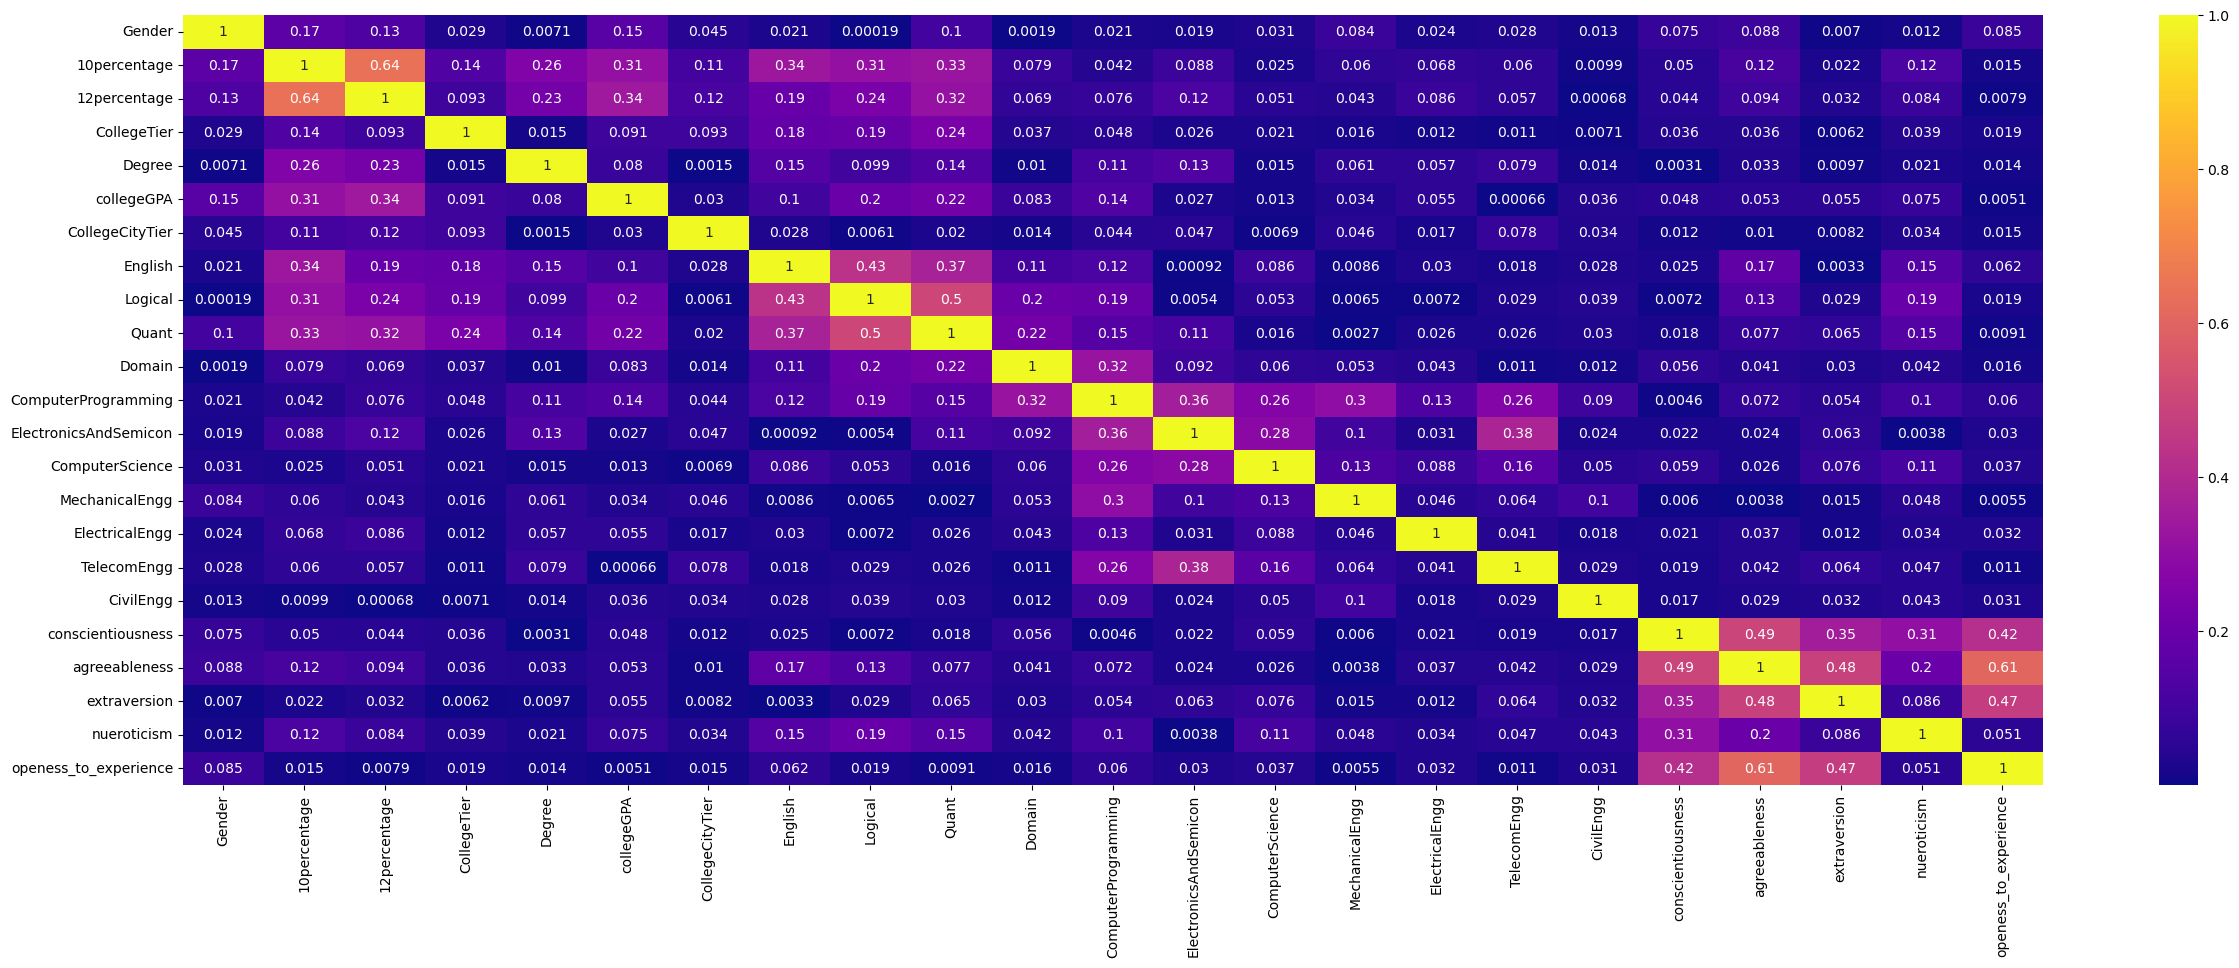
\includegraphics[width=\textwidth]{image/heatmap.png}
    \caption{Ma trận tương quan giữa các cột trong yêu cầu 1d}
    \label{fig:1d_corr}
\end{figure}

\subsubsection{Hàm pandas.corr}
\noindent
\textbf{Input:} Các tham số để tùy chỉnh cách tính ma trận tương quan. \\
\textbf{Output:} DataFrame chứa ma trận tương quan giữa các cột.
\paragraph{Mô tả:}

Ma trận tương quan (correlation matrix) là một ma trận vuông chứa các hệ số tương quan giữa nhiều biến. Mỗi ô trong bảng cho biết mối tương quan giữa hai biến cụ thể. Ma trận tương quan thường được sử dụng để tóm tắt dữ liệu, làm đầu vào cho phân tích nâng cao hơn và làm chẩn đoán cho phân tích nâng cao

Một số điểm cần lưu ý khi đọc ma trận tương quan:
\begin{itemize}
  \item Các hệ số tương quan trên đường chéo của bảng đều bằng 1 vì mỗi biến hoàn toàn tương quan với chính nó.
  \item Chỉ một nửa của ma trận tương quan cần được hiển thị vì nửa còn lại của các hệ số tương quan trong ma trận là dư thừa và không cần thiết.
  \item Ta có thể tô màu ma trận tương quan sẽ được như một bản đồ nhiệt (sử dụng tham số \textit{cmap} trong hàm heatmap) để làm cho các hệ số tương quan dễ đọc hơn.
\end{itemize}

Trong đồ án này, phương pháp Pearson \cite{wikipediaPearsonCorrelation} được sử dụng để tính ma trận tương quan. Phương pháp này được sử dụng để đo lường mối quan hệ giữa hai biến ngẫu nhiên X và Y. Giá trị của hệ số tương quan Pearson nằm trong khoảng [-1, 1]. Hệ số tương quan bằng 1 nếu có mối quan hệ tuyến tính thuận hoàn hảo giữa hai biến, bằng -1 nếu có mối quan hệ tuyến tính nghịch hoàn hảo giữa hai biến. Hệ số tương quan bằng 0 nếu không có mối quan hệ tuyến tính giữa hai biến.

Công thức tính hệ số tương quan Pearson giữa hai biến X và Y:
\begin{equation}
    \text{r}_{\text{X,Y}} = \frac{\sum_{i=1}^{n} (x_i - \bar{x})(y_i - \bar{y})}{\sqrt{\sum_{i=1}^{n} (x_i - \bar{x})^2} \sqrt{\sum_{i=1}^{n} (y_i - \bar{y})^2}}
\end{equation}

Trong đó:
\begin{itemize}
    \item $\text{r}_{\text{X,Y}}$ là hệ số tương quan Pearson giữa hai biến X và Y.
    \item $x_i$ là giá trị của biến X tại điểm dữ liệu thứ i.
    \item $y_i$ là giá trị của biến Y tại điểm dữ liệu thứ i.
    \item $\bar{x}$ là giá trị trung bình của biến X.
    \item $\bar{y}$ là giá trị trung bình của biến Y.
    \item n là số lượng điểm dữ liệu.
\end{itemize}

Do ta cần quan tâm độ tương quan giữa hai đặc trưng chứ không quan tâm chúng có tương quan thuận hay nghịch, nên ta sẽ lấy giá trị tuyệt đối của hệ số tương quan Pearson để tính ma trận tương quan. Bằng cách gọi hàm \textit{abs()} trên DataFrame chứa ma trận tương quan, ta sẽ được ma trận tương quan giữa các cột như hình \ref{fig:1d_corr}.

% Numpy
\subsubsection{Hàm numpy.linalg.inv}
\noindent
\textbf{Input:} Ma trận vuông cần tính ma trận nghịch đảo. \\
\textbf{Output:} Ma trận nghịch đảo của ma trận đầu vào.
\paragraph{Mô tả:}

Hàm \textit{numpy.linalg.inv} \cite{numpyNumpylinalginv} được sử dụng để tính ma trận nghịch đảo của ma trận vuông. Trong đồ án này, hàm này được sử dụng để tính ma trận nghịch đảo của ma trận $\text{A}^\text{T} \text{A}$ để tìm nghiệm của hệ phương trình tuyến tính $\text{x} = (\text{A}^\text{T} \text{A})^{-1} \text{A}^\text{T} \text{b}$ (hàm \textit{fit} trong class OLSLinearRegression tự cài đặt, song để tối ưu hoá thời gian tính toán, ta sẽ sử dụng hàm \textit{numpy.linalg.inv} để tính ma trận nghịch đảo thay vì tự cài đặt).

\subsubsection{Hàm numpy.ravel}
\noindent
\textbf{Input:} Mảng NumPy được đọc theo thứ tự được chỉ định bởi tham số order và được đóng gói thành một mảng 1 chiều và được đọc theo thứ tự C. \\
\textbf{Output:} Mảng NumPy một chiều.
\paragraph{Mô tả:}

Trong numpy, tham số order được sử dụng để chỉ định cách mà các phần tử của một mảng được lưu trữ trong bộ nhớ C trong \textit{order='C'}, có nghĩa là mảng được lưu trữ theo thứ tự liên tục của C, hay chỉ số cuối cùng thay đổi nhanh nhất \cite{stackoverflowCOrder}. Điều này có nghĩa là khi bạn duyệt qua các phần tử của một mảng nhiều chiều theo thứ tự C, bạn sẽ duyệt qua các phần tử của chỉ số cuối cùng trước, sau đó tăng chỉ số kế cuối lên 1 và tiếp tục duyệt qua các phần tử của chỉ số cuối cùng, và cứ tiếp tục như vậy cho đến khi duyệt hết các phần tử của mảng.

Trong bài toán hồi quy tuyến tính, chúng ta cần tìm một ma trận trọng số self.w sao cho tổng bình phương sai số giữa giá trị dự đoán và giá trị thực tế là nhỏ nhất. Để làm được điều này, chúng ta cần biến đổi ma trận trọng số thành một vector có kích thước bằng với số lượng tham số trong mô hình. Hàm \textit{numpy.ravel()} \cite{numpyNumpyravel} giúp chúng ta thực hiện việc này một cách dễ dàng và nhanh chóng. Bằng cách sử dụng hàm này, chúng ta có thể tính toán tích vô hướng giữa vector trọng số và ma trận đầu vào X bằng cách nhân từng phần tử tương ứng và cộng lại bằng cách gọi hàm \textit{numpy.sum}. Cuối cùng ta thu được giá trị dự đoán cho từng quan sát trong ma trận đầu vào X.

Hàm \textit{numpy.ravel} cũng được sử dụng trong hàm mae \ref{mae} để làm phẳng các mảng đầu vào y và y\_hat thành các mảng 1 chiều. Điều này cho phép tính toán trực tiếp sự khác biệt tuyệt đối giữa các phần tử tương ứng của hai mảng bằng cách trừ chúng và lấy giá trị tuyệt đối. Sau đó, giá trị trung bình của các sự khác biệt tuyệt đối được tính toán bằng hàm \textit{numpy.mean} để trả về giá trị lỗi trung bình tuyệt đối (MAE) giữa hai mảng.

\subsubsection{Hàm numpy.sum}
\subsubsection{Hàm numpy.mean}
\subsubsection{Hàm numpy.triu}
\subsubsection{Hàm numpy.where}
\subsubsection{Hàm numpy.ones}
% Seaborn
\subsubsection{Hàm seaborn.heatmap}
% Sklearn
\subsubsection{Hàm sklearn.model\_selection.KFold}
% IPython
\subsubsection{Hàm IPython.display.Latex}

\subsection{Hàm tự cài đặt}
\subsubsection{Hàm OLSLinearRegression.fit}
\subsubsection{Hàm OLSLinearRegression.predict}
\subsubsection{Hàm OLSLinearRegression.get\_params}
\subsubsection{Hàm mae} \label{mae}
\subsubsection{Hàm latex\_text}
\subsubsection{Hàm kfold\_cross\_model}
\subsubsection{Hàm scientific\_notation\_converter}

\section{Đánh giá kết quả mô hình}
\subsection{Yêu cầu 1a}

\subsection{Yêu cầu 1b}

\subsection{Yêu cầu 1c}

\subsection{Yêu cầu 1d}

\newpage
\printbibliography[heading=mybibintoc]

\end{document}